\section{Conditional torque consistency on the multi-speed reference}
\label{sec:real-torque}
\subsection{Selection and qualification of the comparison channel}
A useful real example must separate a numerical calculation from the
qualification of its observations. A repository-wide MAT-file inventory,
deduplicated by SHA-256, finds two distinct measurement files.
Their actual signal lists contain averaged dq currents and voltages,
operating indices, speed, temperature references, and
\texttt{CAN\_Torque\_meas}, but no directly recorded dq flux arrays.
Thus the fluxes here are reconstructed electrical samples, not independently
measured flux ground truth. The multi-speed file
\texttt{WW\_Dataset\_Multi\_RPM.mat} supplies the primary example;
the outlier file is not used to qualify the torque law.
The chosen file has repeat observations and shared requested-current
support at two speeds, while the outlier file's CAN range is much broader.

Signal provenance is traced through the existing MATLAB v7.3 importer and
the raw HDF5 recorder metadata. The CAN channel's \texttt{Unit} and
\texttt{Description} are empty. Its \texttt{Device} is \texttt{Platform}
and its path ends in
\texttt{Recorder/Data\_Recorder/Recorder Values}.
Recording metadata identify ControlDesk and a DS1202 MicroLabBox software
revision, but the defining model/signal description is not supplied.
No transducer location, sensor calibration, torque unit, gain, offset,
loss compensation, or motor/generator sign definition is recoverable.
Torque request channels are zero; this does not establish the measured
channel's meaning. In particular neither electromagnetic nor shaft torque
is proven by its name.

We denote the recorded comparison channel by $\cantorqueindicator$ and,
solely for the numerical demonstration, interpret its numeric values as
Nm with unity gain and their recorded sign. The conditional residuals are
\begin{equation}
 e_M^{\rm CAN}=M_{\rm map}-M_{\rm CAN},\qquad
 e_{\psi_\tau}^{\rm CAN}=\frac{e_M^{\rm CAN}}{k_{\rm T}I_s}.
 \label{eq:conditional-can-residual}
\end{equation}
The superscript records this assumption. We do not set
$M_{\rm em,ref}=M_{\rm CAN}$. Even describing it as measured shaft torque
would exceed the available provenance. Failure of the qualification gate
permits a consistency demonstration under a stated conversion hypothesis,
not experimental validation of electromagnetic torque or of a flux correction.

\subsection{Matched reduction, stationarity, and conditioning}
Requested 1000 and 3000 rpm and a rotor-temperature reference of
70 $^\circ$C select two slices. Each has 327 finite records in 109
operating-index groups. The existing loader uses configured $p=4$,
$R_s=\SI{10}{\milli\ohm}$, and requested
$\omega_e=2\pi pn/60$ for voltage inversion. CAN, measured current,
voltage, and recorded speed are averaged on the same indices;
each OP group has equal weight. No residual filter, sign reversal,
gain fit, resistance adjustment, or interpolation is applied.
The multiplication uses the same measured mean currents that label
the reconstructed flux vectors.

\Cref{tab:torque-support} reports recorded speed support and repeat scatter.
The independent \texttt{CAN\_RPM\_meas} channel is identically zero,
whereas \texttt{PE\_speed\_rpm} is close to the requested speeds.
Neither approximate speed agreement nor three repeated records proves
zero acceleration within the averaging windows. The recorder's increasing
X array has an empty unit; window definitions and sensor synchronization
are unspecified. We therefore do not infer a calibrated $J_m\dot\omega_m$
from finite differences of these reduced data.
\begin{table}[tb]
 \centering\small
 \begin{tabular}{rrrrrr}
\toprule
$n$ & $I_{\min}$ (A) & Retained & CAN SD & Speed range (rpm) & OP speed SD\\
\midrule
1000 & 10.02 & 108 & 0.492 & 984.36--1015.24 & 4.084\\
3000 & 10.04 & 108 & 0.269 & 2984.97--3013.38 & 2.601\\
\bottomrule
\end{tabular}

 \caption{Generated support at the 70-$^\circ$C rotor reference. CAN SD
 is the median sample standard deviation of three records per OP,
 conditionally in Nm; OP speed SD is its analogous median in rpm.
 These are descriptive repeat scatters, not calibrated standard errors.}
 \label{tab:torque-support}
\end{table}

Normalize only for $I_s>0.10 I_{s,\max}$ in each slice. This caps the
torque-noise conversion at ten times its full-current value; it is a
conditioning policy, not a sensor-resolution claim. It excludes the
near-origin group and retains 108 OP groups at each speed.
The unnormalized torque residual retains all groups. Fractions
0.05, 0.15, and 0.20 are also evaluated: 0.05 has the same support,
and the higher thresholds preserve the dominant spatial pattern.
Full quantiles and threshold sensitivities are stored in the reproducible
JSON, rather than selecting a threshold to minimize the residual.

Rotor and stator temperature references are constant in this dataset;
they do not establish measured winding equilibrium or support a thermal
dependence study. The excitation request is zero and recorded
\texttt{I\_exc\_meas} has only a small near-zero range of unverified origin.
There is no controlled excitation sweep from which to infer an EESM
dependence or even to establish machine type. The projection result
applies to an excitation slice, but no real excitation effect is claimed.

\subsection{Spatial disagreement dominates the mean bias}
\Cref{tab:torque-metrics} separates signed summaries from error magnitudes.
The small signed bias coexists with large conditional RMS disagreement
because opposite current directions cancel in the mean.
\begin{table}[tbp]
 \centering\small
 \begin{tabular}{rrlrrrrrr}
\toprule
$n$ & $N$ & Residual & Bias & MAE & RMSE & Median & $q_{05}$ & $q_{95}$\\
\midrule
1000 & 109 & $e_M^{\rm CAN}$ (Nm) & 0.998 & 16.489 & 19.665 & 1.262 & -29.340 & 31.686\\
1000 & 108 & $e_{\psi_\tau}^{\rm CAN}$ (mWb) & 2.775 & 37.828 & 41.960 & 2.794 & -52.830 & 56.966\\
3000 & 109 & $e_M^{\rm CAN}$ (Nm) & 1.415 & 16.430 & 19.572 & 1.590 & -29.001 & 31.878\\
3000 & 108 & $e_{\psi_\tau}^{\rm CAN}$ (mWb) & 4.209 & 37.918 & 41.943 & 4.219 & -51.742 & 58.209\\
\bottomrule
\end{tabular}

 \caption{Generated OP-weighted conditional CAN residuals. $n$ is rpm;
 $N$ is retained OP count. Bias is mean signed residual; MAE and RMSE
 quantify magnitude. Quantiles use the empirical linear interpolation
 convention. All torque units assume CAN numeric values are Nm.}
 \label{tab:torque-metrics}
\end{table}
\Cref{fig:torque-real-maps} preserves actual measured support.
For positive $i_q$ the conditional residual is predominantly negative;
for negative $i_q$ it is predominantly positive. Its torque magnitude grows
with current magnitude, while flux normalization exposes a direction-dependent
pattern reproduced at both speeds. Support lies mainly in the negative-d
half-plane; the plot supplies no validation in unmeasured quadrants.
The shared row maxima are 36.27 conditional Nm and 60.44 conditional mWb. 
\begin{figure}[tbp]
 \centering
 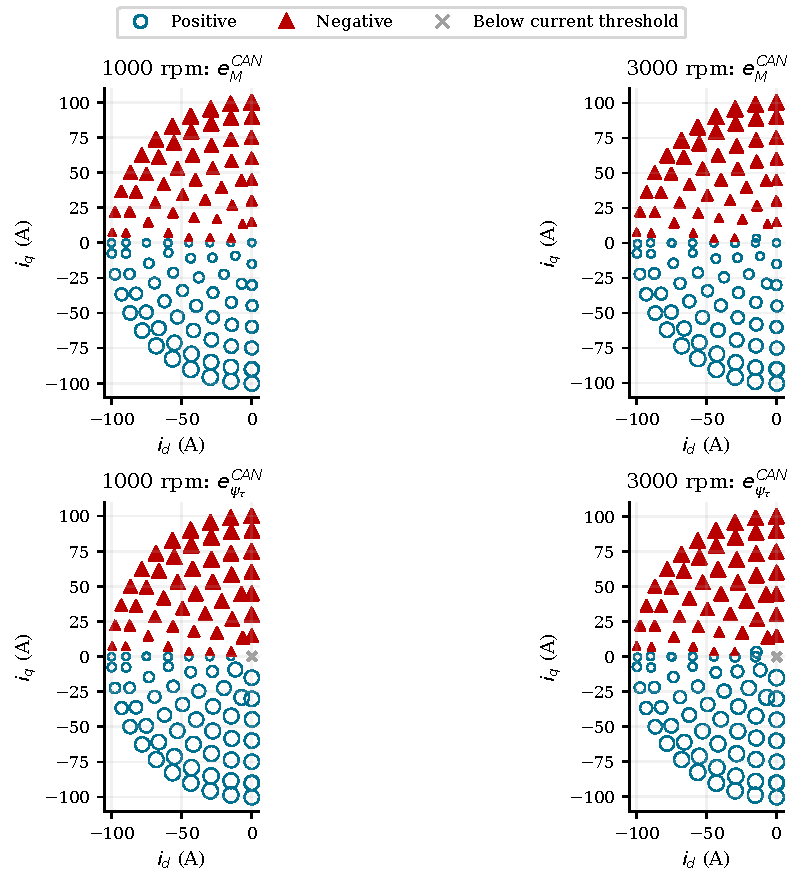
\includegraphics[width=.90\textwidth]{figures/08_torque_real_maps.pdf}
 \caption{Conditional CAN residuals at measured OP coordinates, without
 spatial interpolation. Top: torque residual, all groups. Bottom:
 torque-equivalent flux residual above the current threshold.
 Circle/triangle shapes encode sign; marker area above a fixed visibility
 floor is proportional to absolute residual on a common scale within each row.
 Crosses mark omitted
 normalized values. CAN-to-Nm conversion and dq scaling are assumptions,
 so these maps show consistency disagreement, not identified flux error.}
 \label{fig:torque-real-maps}
\end{figure}

\Cref{fig:torque-real-trends} makes the distinction between bias and
structure explicit. The CAN-versus-map cloud is approximately linear
but departs strongly from the equality line, and the normalized
residual varies predominantly with current direction.
The median CAN-to-map ratio on $|M_{\rm map}|\ge\SI{10}{\newton\metre}$ is 2.005 at 1000 rpm and 1.989 at 3000 rpm. This describes a scale-like disagreement; it is not an identified gain. Replacing requested speed by the mean recorded speed changes $M_{\rm map}$ by RMS \SI{0.056}{\newton\metre} and \SI{0.025}{\newton\metre}, respectively. The RMS difference between torque of mean inputs and mean torque of sample inputs is $ 7.92\cdot10^{-5}$ and $ 2.77\cdot10^{-4}$ Nm, respectively. Neither sensitivity accounts for the conditional discrepancy.

On 104 common requested-current keys, the 3000-minus-1000-rpm conditional torque residual has mean \SI{0.414}{\newton\metre} and RMS \SI{0.717}{\newton\metre}. This is a comparison at matched requested labels, not identical measured current or magnetic state.

The similar large directional pattern at both speeds is not consistent
with explaining all of it by a sole fixed resistance mismatch, whose
torque contribution at matched current would scale as $1/\omega_e$.
It is compatible with several alternatives, including unverified torque
scaling or an incorrect dq convention. For voltage-inverted flux, the
configured $p$ cancels between $k_{\rm T}$ and requested $\omega_e$;
changing that value alone cannot resolve this comparison. Approximate
current-RMS scaling is not an independent voltage or torque calibration.
No scale correction is inferred.
\begin{figure}[tbp]
 \centering
 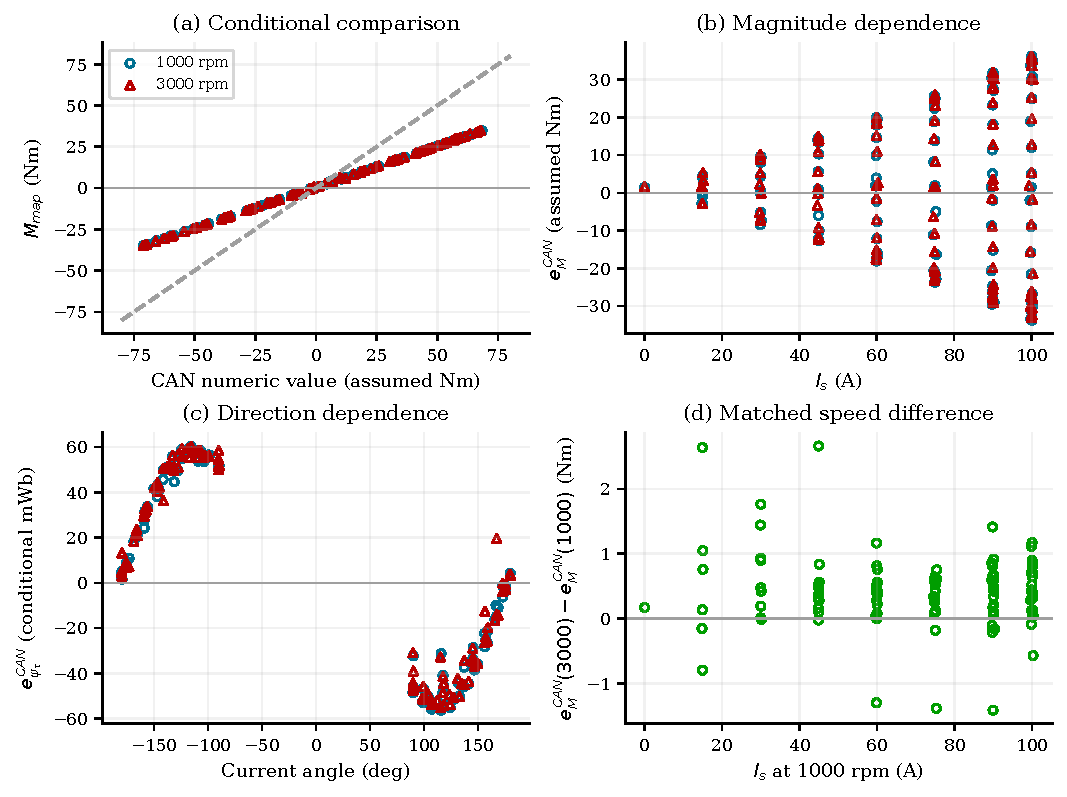
\includegraphics[width=\textwidth]{figures/09_torque_real_trends.pdf}
 \caption{Conditional CAN comparison, magnitude and angle dependence,
 and matched-label speed differences. Open circles and triangles identify
 the two speeds. The diagonal in (a) is equality, not a fitted calibration.
 Panel (d) averages repeated requested-current keys before matching;
 equal requested labels need not have equal measured currents.}
 \label{fig:torque-real-trends}
\end{figure}

The results establish that the real observation channel contains a
reproducible spatial disagreement under the declared conversion.
They do not establish which map, sensor, loss term, or convention is wrong.
Dataset and source hashes, signal metadata, unfiltered OP tables,
matched-speed tables, binned current/angle summaries, and generated figures
are produced by \texttt{numerics/torque\_consistency.py}.
